\documentclass{article}

\usepackage{graphicx}
\usepackage[colorlinks,linkcolor=blue]{hyperref}

\begin{document}
    \title{\textbf{TransportIDE} -- An integrated transportation system design and test environment}
    \author{Georg Hackenberg}
    \maketitle
    
    \begin{abstract}
        Due to many reasons transportation systems have to become more and more efficient.
        This observation holds true both for person transport and for good transport, on public infrastructure and on private infrastructure.
        Designing efficient transportation systems is a difficult undertaking due to the vast size of the solution space and the emergent dynamics of the system components.
        Transportation system designers need appropriate tools to explore the design space and test solutions quickly and reliably.
        In this paper, we propose a simulation-based environment for transportation system design and test, which is built on a solid system theory.
        Furthermore, we demonstrate possible applications such as comparison of different infrastructure and control algorithm designs.
    \end{abstract}
    
    \section{Introduction}
    \label{sec:intro}
    TODO~\cite{key}

    \subsection*{Research question}
    How can we support the design and test of transportation infrastructures and control algorithms better?
    Which modeling and simulation technique represents an appropriate abstraction for the domain?
    Which software architecture is appropriate for an integrated design and test environment?
    Which application scenarios should be supported on top of this environment?

    \subsection*{Research methodology}
    To answer the above questions, we apply and combine two research methodologies.
    First we conduct a literature review to understand the state of the art in transportation system design and test.
    Second we use iterative and incremental software development with regular feedback from stakeholders to develop our a new dedicated approach.

    \subsection*{Document outline}
    In the following, w e first present related work on transportation system design and test in Section~\ref{sec:related}.
    Then we describe the underlying system theory of our approach in Section~\ref{sec:theory}.
    Afterwards, we explain our software architecture in Section~\ref{sec:arch}.
    Thereafter, we demonstrate three software applications in Section~\ref{sec:app}.
    Finally, we draw our conclusion in Section~\ref{sec:con}.

    \section{Related work}
    \label{sec:related}
    TODO

    \section{System theory}
    \label{sec:theory}
    TODO

    \section{Software architecture}
    \label{sec:arch}
    TODO Figure~\ref{fig:0}

    \begin{figure}
        \centering
        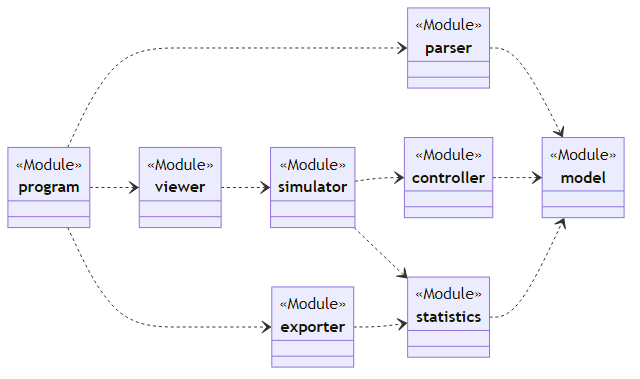
\includegraphics[width=0.7\textwidth]{../../diagrams/architecture.png}
        \caption{Module architecture}
        \label{fig:0}
    \end{figure}

    \subsection{Model}
    TODO Figure~\ref{fig:1}

    \begin{figure}
        \centering
        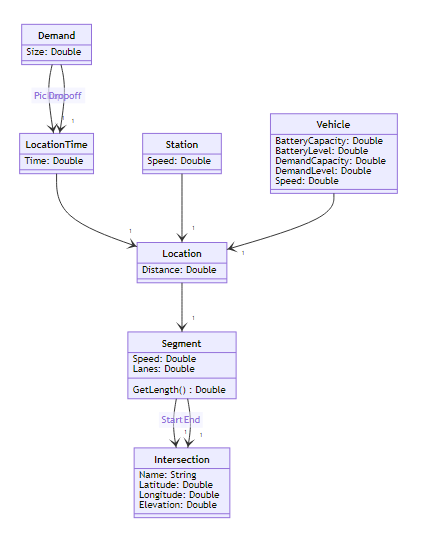
\includegraphics[width=\textwidth]{../../diagrams/model/classes-v0.png}
        \caption{Data model}
        \label{fig:1}
    \end{figure}

    \subsection{Controller}
    TODO Figure~\ref{fig:2}

    \begin{figure}
        \centering
        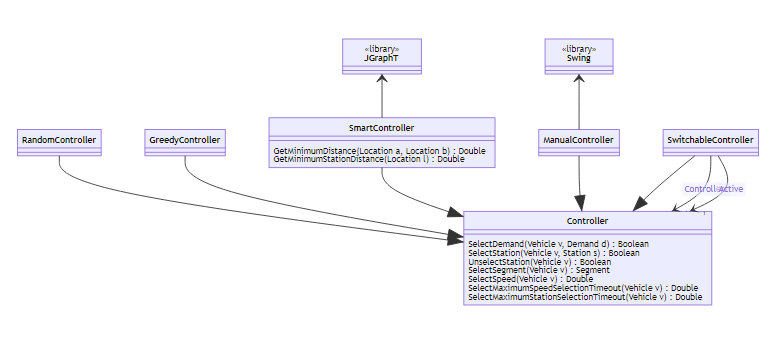
\includegraphics[width=\textwidth]{../../diagrams/controller/classes.png}
        \caption{Controller interface}
        \label{fig:2}
    \end{figure}

    \subsubsection{Manual}
    TODO

    \subsubsection{Random}
    TODO
    
    \subsubsection{Greedy}
    TODO

    \subsubsection{Smart}
    TODO

    \subsubsection{Switchable}
    TODO

    \subsection{Statistics}
    TODO Figure~\ref{fig:3}

    \begin{figure}
        \centering
        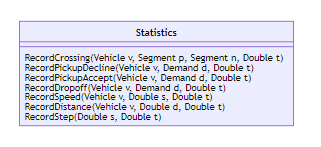
\includegraphics[width=0.5\textwidth]{../../diagrams/statistics/classes.png}
        \caption{Statistics interface}
        \label{fig:3}
    \end{figure}

    \section{Software application}
    \label{sec:app}
    TODO

    \subsection{Basic simulation}
    TODO Figure~\ref{fig:4}

    \begin{figure}
        \centering
        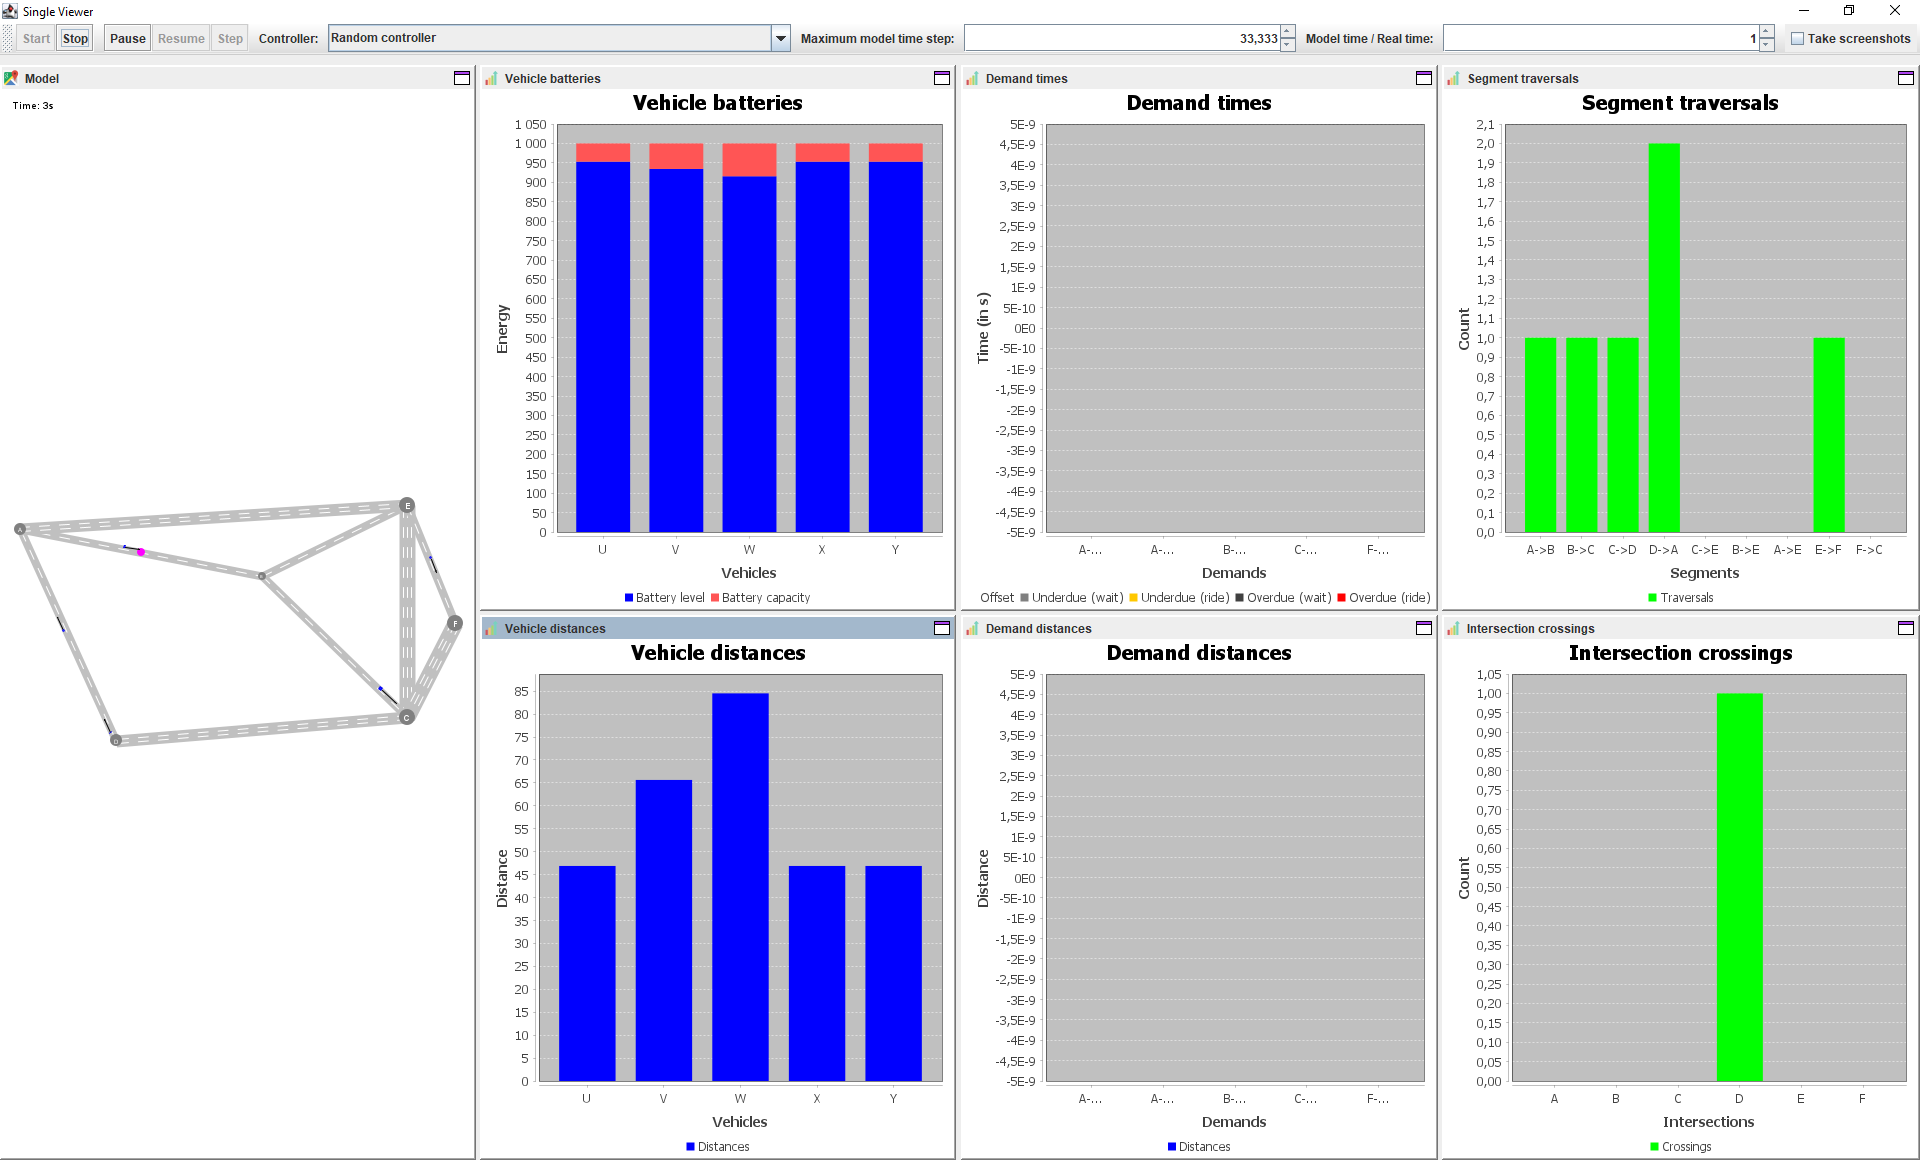
\includegraphics[width=\textwidth]{../../screenshots/basic-simulation.png}
        \caption{Basic simulation}
        \label{fig:4}
    \end{figure}

    \subsection{Controller comparison}
    TODO Figure~\ref{fig:5}

    \begin{figure}
        \centering
        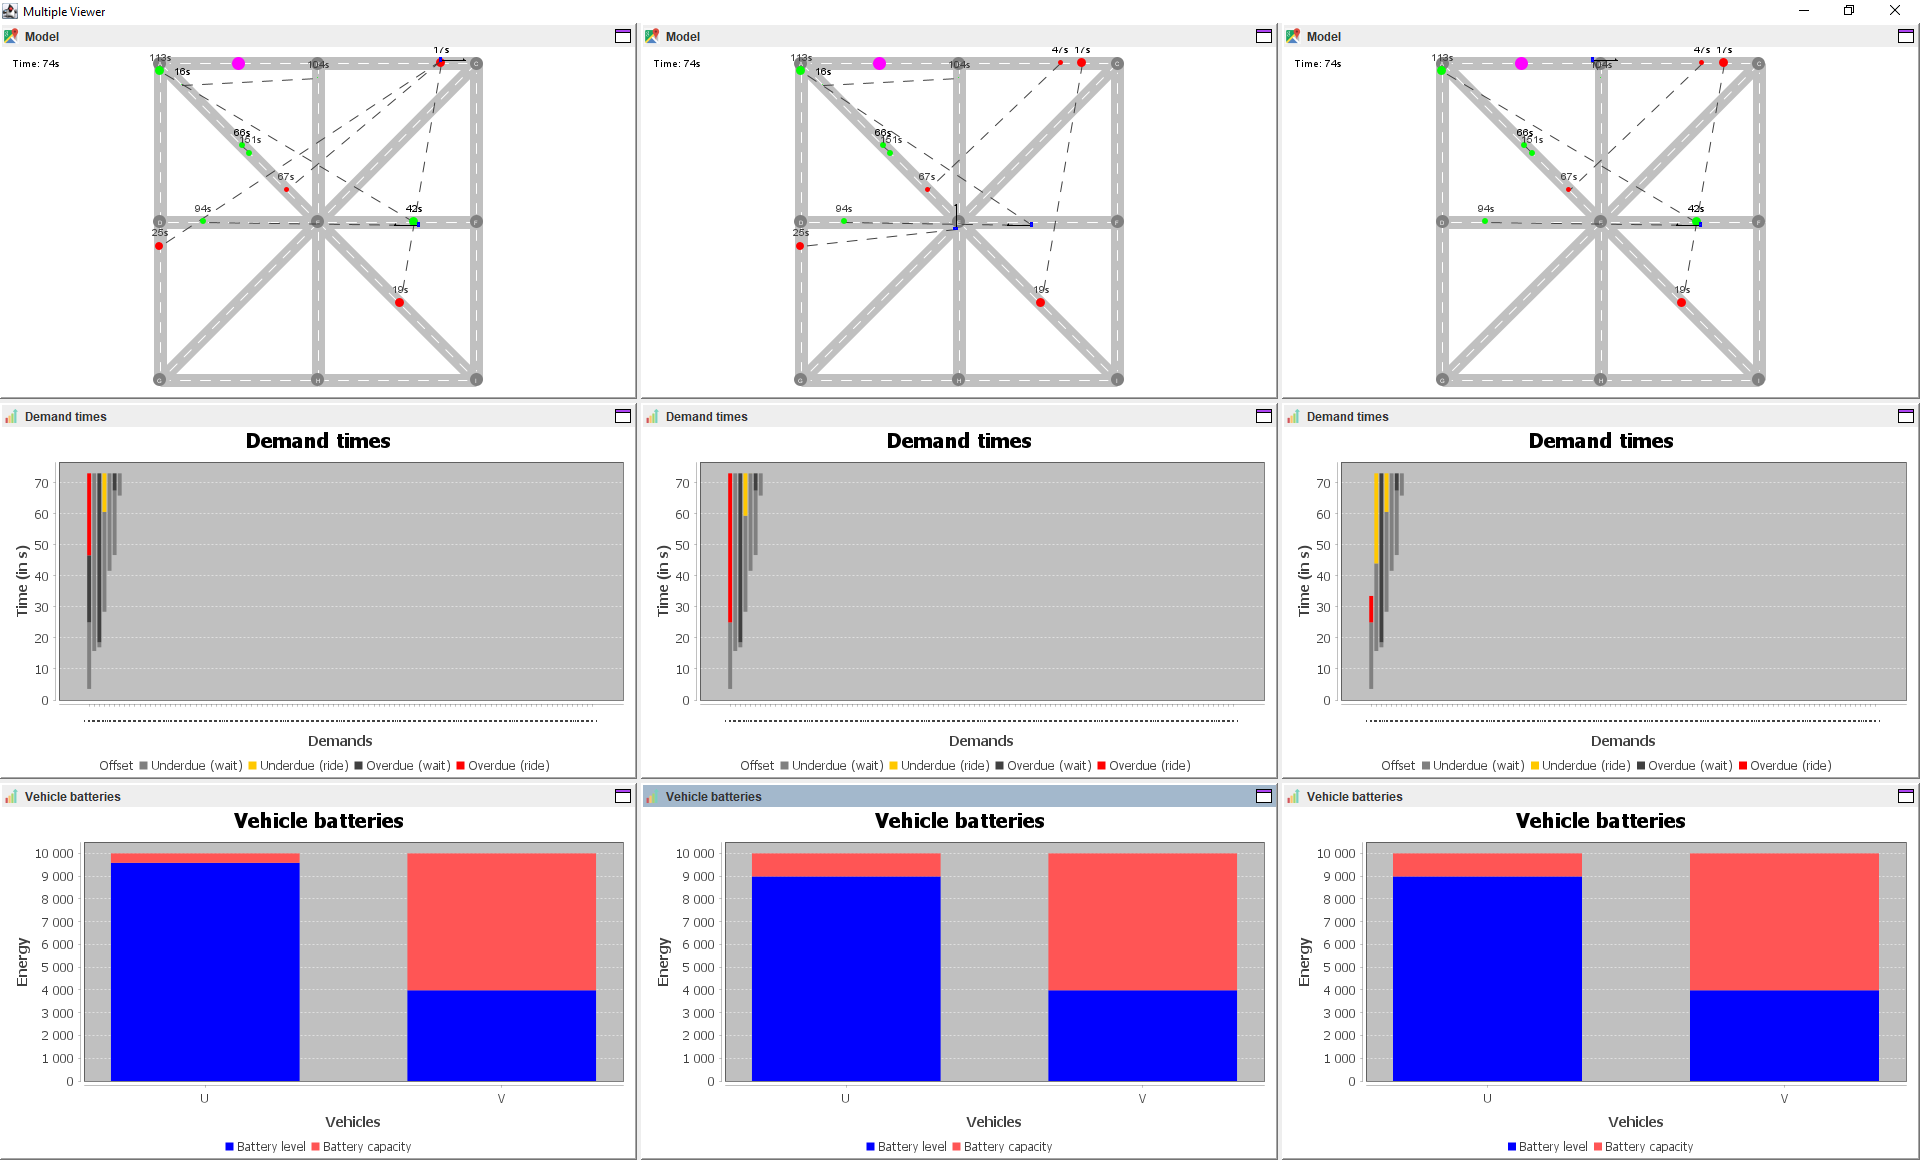
\includegraphics[width=\textwidth]{../../screenshots/controller-comparison.png}
        \caption{Controller comparison}
        \label{fig:5}
    \end{figure}

    \subsection{Infrastructure comparison}
    TODO Figure~\ref{fig:6}

    \begin{figure}
        \centering
        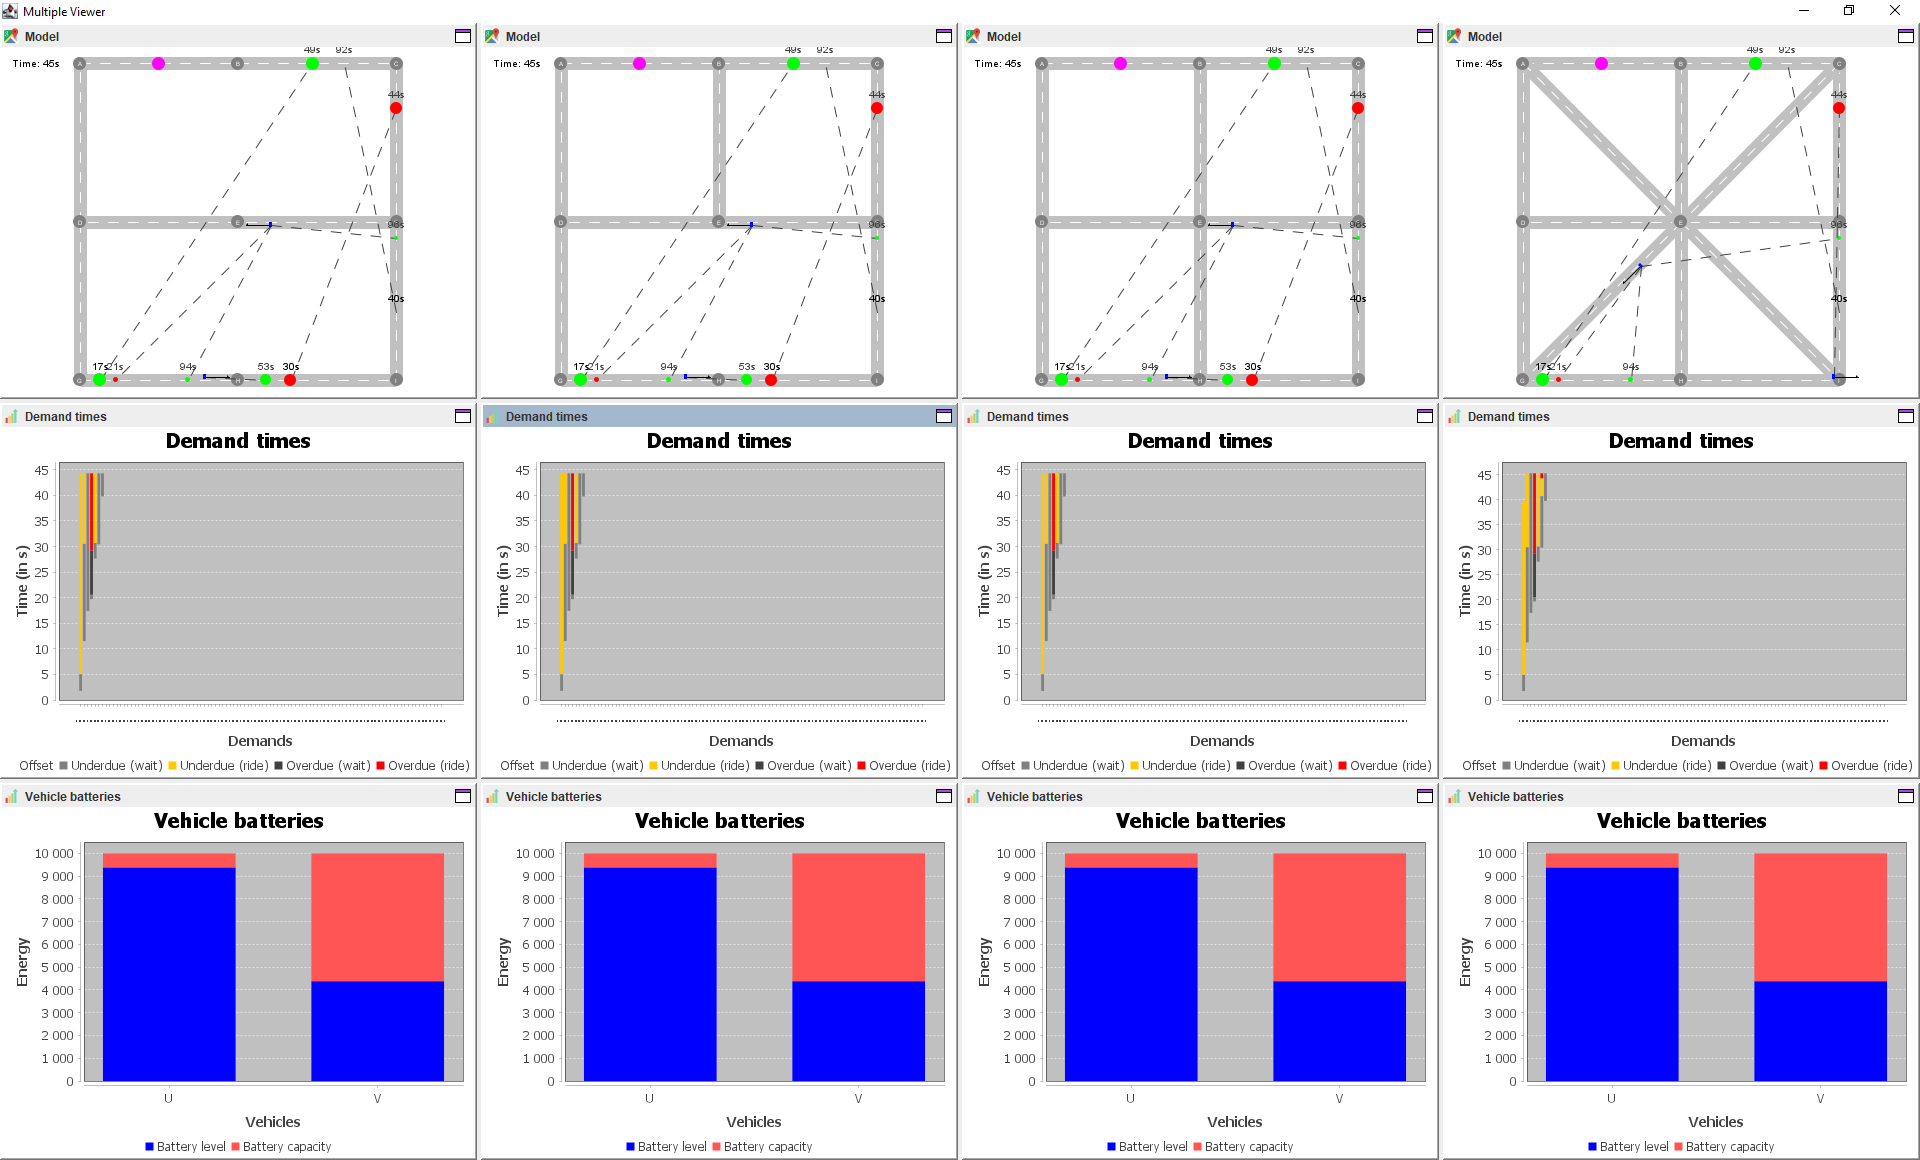
\includegraphics[width=\textwidth]{../../screenshots/infrastructure-comparison.png}
        \caption{Infrastructure comparison}
        \label{fig:6}
    \end{figure}

    \section{Conclusion}
    \label{sec:con}
    TODO

    \bibliographystyle{plain}
    \bibliography{main}
\end{document}